\chapter{Experiments} \label{chap:experiments}

In this chapter, we explain the setup of our experiments, describe how we measure the performance of different methods, and present the results. All experiments were performed using either the AMD EPYC 9454 or the AMD EPYC 9474F CPUs.

\section{Datasets}

Here we briefly describe all datasets provided with the Google Hash Code Traffic signaling problem. This is important because the datasets have different sizes and structures.

\paragraph{A - An example: 4 parameters} Simple toy problem dataset used for debugging (See Figure~\ref{fig:hashcode_dataset_a}).

\paragraph{B - By the ocean: 5,974 parameters} Dataset based on a real city plan of Lisbon, Portugal (See Figure~\ref{fig:hashcode_dataset_b}).

\paragraph{C - Checkmate: 14,008 parameters} Dataset with a chessboard-like pattern and regular structure of intersections and streets (See Figure~\ref{fig:hashcode_dataset_c_e}).

% https://codeforces.com/blog/entry/88188#comment-765574
\paragraph{D - Daily commute: 167,748 parameters} By far the largest dataset with a challenging-to-navigate network from the \textit{Barabási-Albert} distribution.

\paragraph{E - Etoile: 1,386 parameters} Nicknamed \textit{Etoile}\footnote{\textit{Étoile} means star in French.}, this dataset is a one big star, meaning there is one very important intersection in the middle with hundrets of incoming streets (See Figure~\ref{fig:hashcode_dataset_c_e}).

\paragraph{F - Forever jammed: 10,002 parameters} Medium sized dataset but again with a complex network difficult to optimize.

\begin{figure}
    \centering
    % 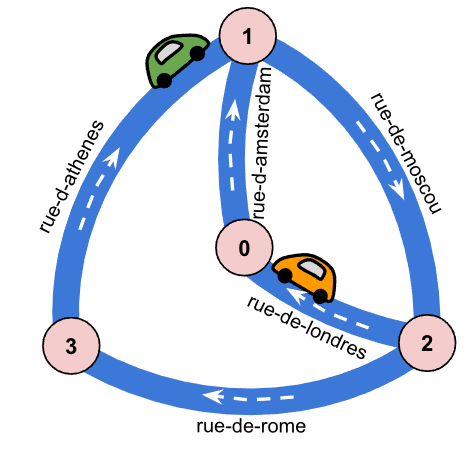
\includegraphics[width=\linewidth]{img/hashcode/figure5.png}
    % 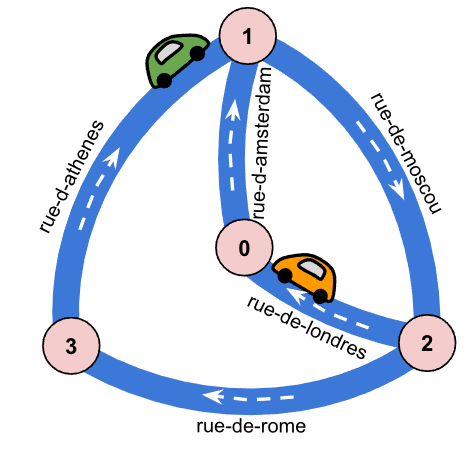
\includegraphics[width=.6\linewidth]{img/hashcode/figure5.png}
    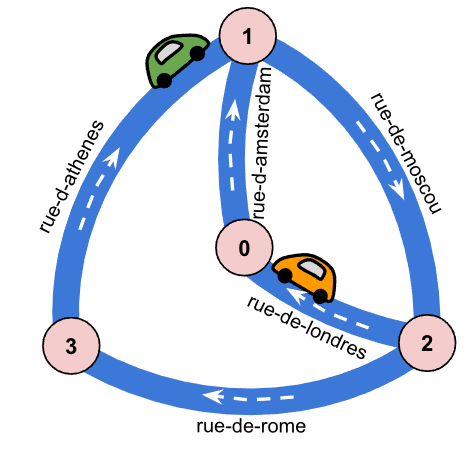
\includegraphics[width=.5\linewidth]{img/hashcode/figure5.png}
    \caption[Visualization of dataset A]{
        Visualization of dataset A \cite{google2023google}.
    }
    \label{fig:hashcode_dataset_a}
\end{figure}

\begin{figure}
    \centering
    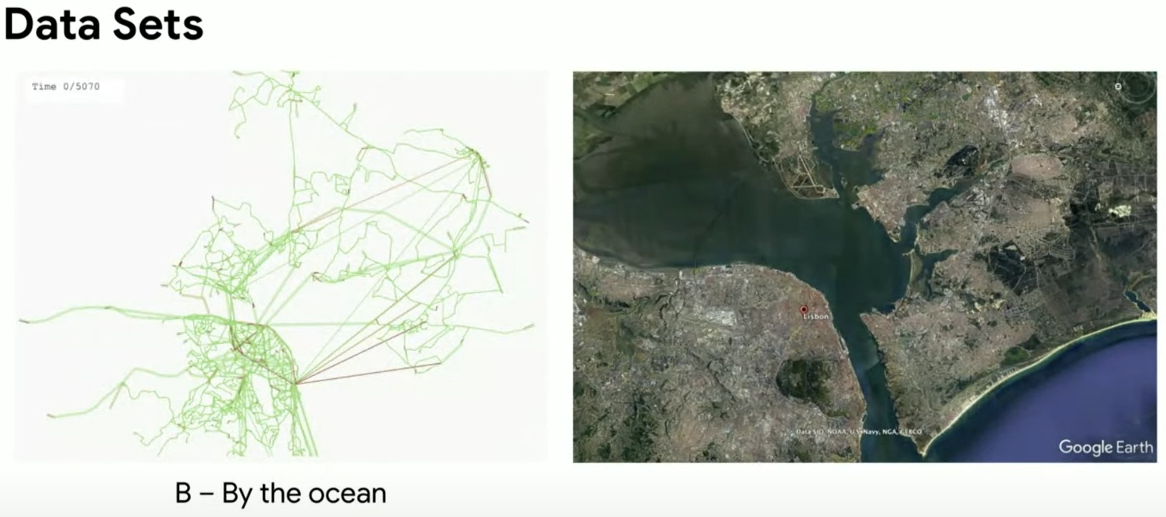
\includegraphics[width=\linewidth]{img/screenshots/hashcode_datasets_b.png}
    % 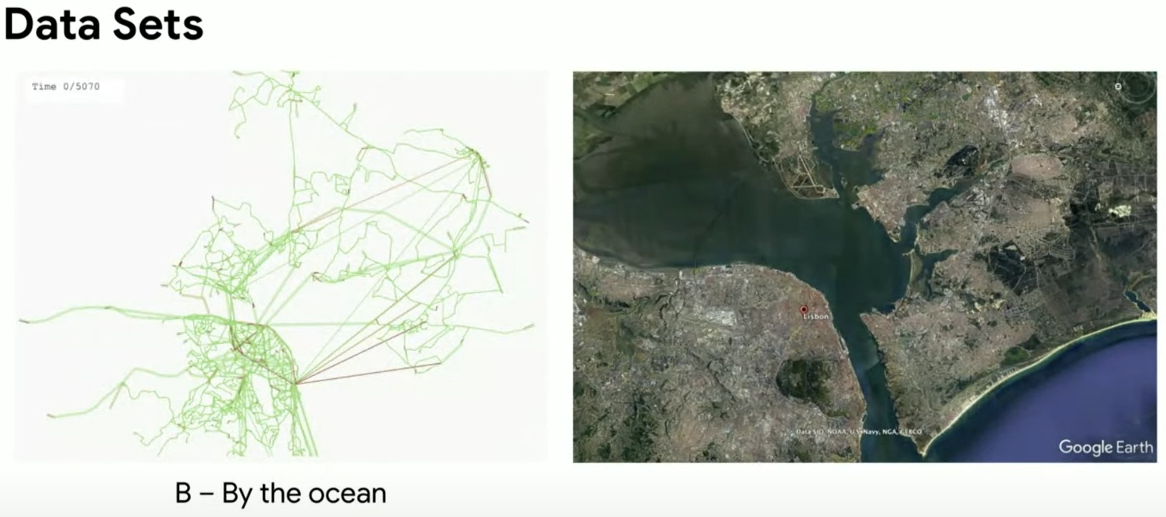
\includegraphics[width=.8\linewidth]{img/screenshots/hashcode_datasets_b.png}
    \caption[Visualization of dataset B]{
        Dataset B based on the real data of Lisbon on the right\footnotemark.
    }
    \label{fig:hashcode_dataset_b}
\end{figure}

\footnotetext{Screenshot from \href{https://www.youtube.com/watch?v=YPOVd-hQUjA}{Hash Code 2021: Online Qualification Round Livestream}.}

\begin{figure}
    \centering
    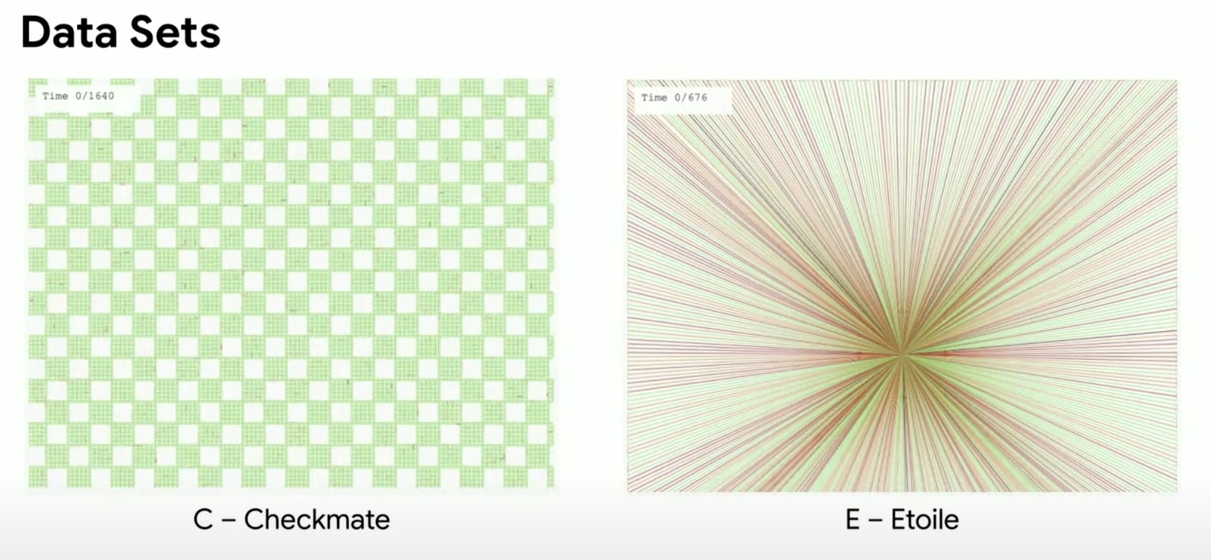
\includegraphics[width=\linewidth]{img/screenshots/hashcode_datasets_c_e.png}
    % 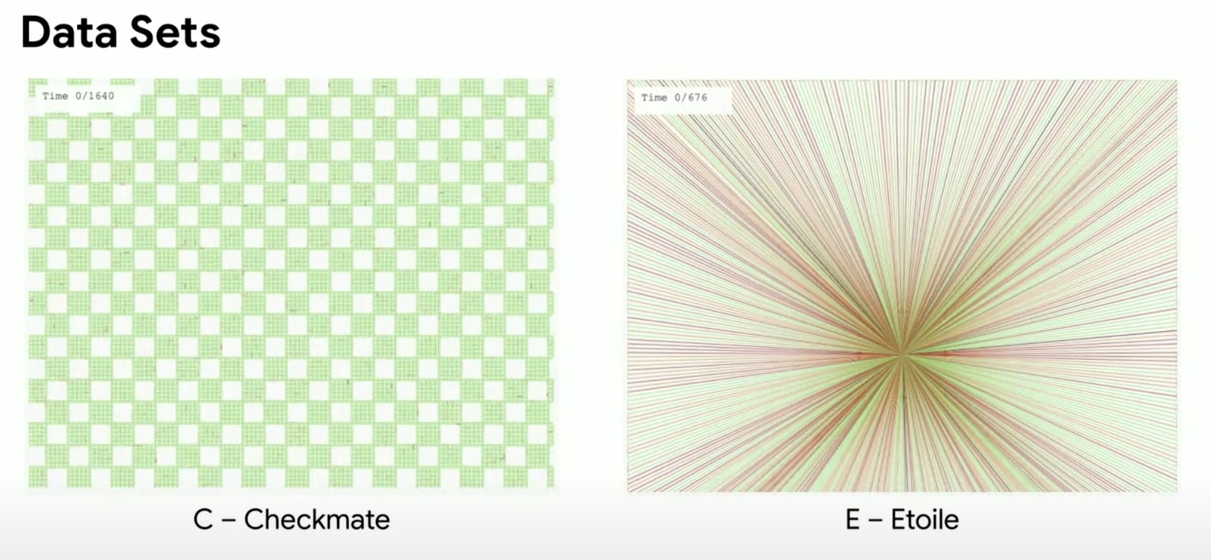
\includegraphics[width=.8\linewidth]{img/screenshots/hashcode_datasets_c_e.png}
    \caption[Visualization of datasets C and E]{
        Datasets C and E\footnotemark.
        }
        \label{fig:hashcode_dataset_c_e}
    \end{figure}
    
\footnotetext{See previous footnote.}

\bigskip

As previously stated, each dataset yields an absolute score in different range. To compare the performance across all datasets, we normalize the scores to a 0--1 range. 0 is a baseline solution with default order and default times and 1 is the maximum known score for the dataset. Note that the baseline is already a good solution and there may not be much room to improve further, e.g., in dataset B.

\section{Experiment 2: Optimization}

In the second experiment, we compare different optimization methods on datasets B--F. The goal is to find if some method is superior to others or if the ideal method is dataset-dependent. We also want to see how much we can improve from the starting solutions.

\subsection*{Methodology}

We compare the three previously mentioned optimization methods: \textit{genetic algorithm}, \textit{hill climbing} and \textit{simulated annealing}. For each dataset and method, 10 runs with different seeds were performed and averaged to obtain reliable results. ...

\subsection*{Results}

\begin{figure}
    \centering
    % 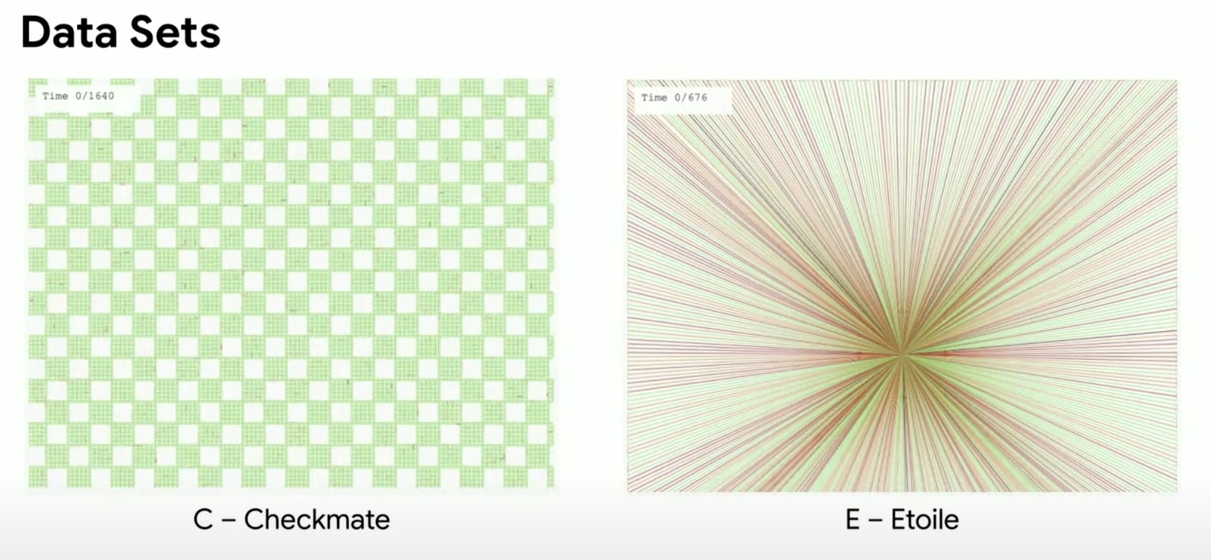
\includegraphics[width=\linewidth]{img/screenshots/hashcode_datasets_c_e.png}
    % 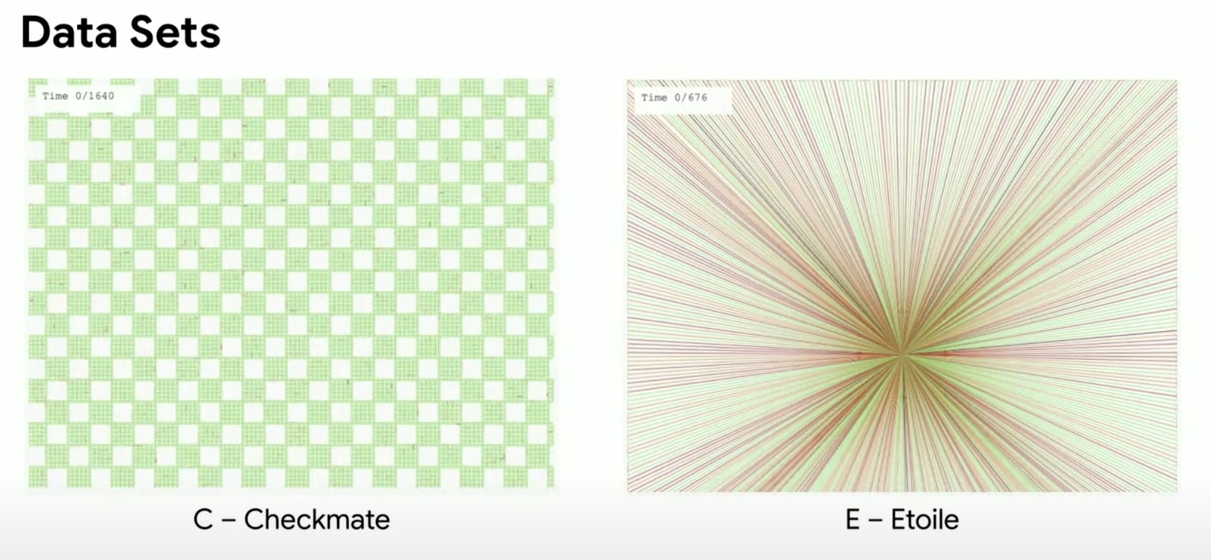
\includegraphics[width=.8\linewidth]{img/screenshots/hashcode_datasets_c_e.png}
    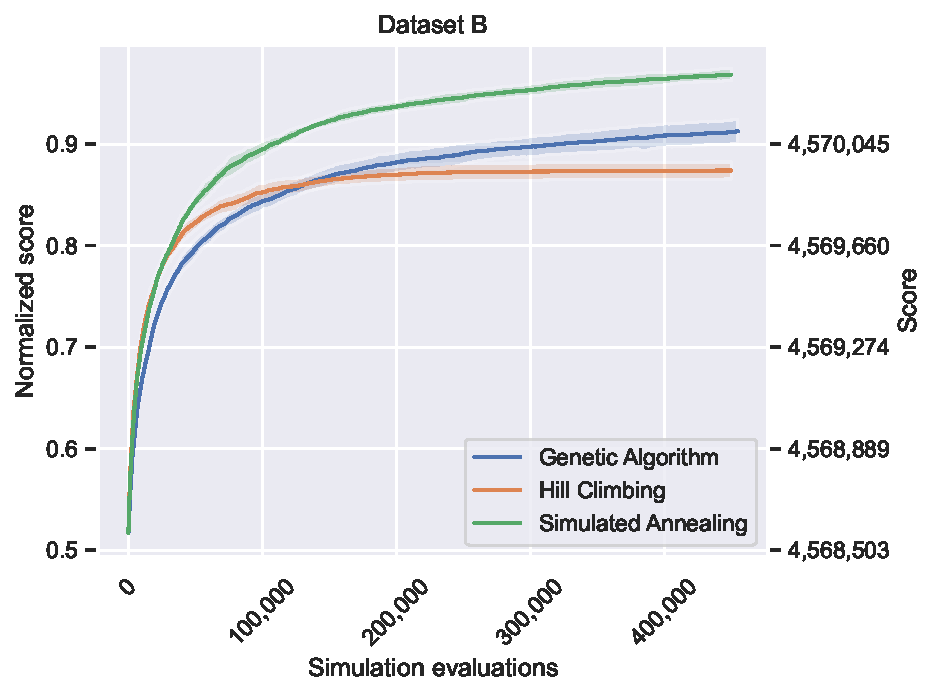
\includegraphics[width=\linewidth]{img/experiments/b_Genetic Algorithm_Hill Climbing_Simulated Annealing.pdf}
    \caption[Results for dataset B]{
        Results for dataset B.
    }
    \label{fig:dataset_b_experiment}
\end{figure}

\begin{figure}
    \centering
    % 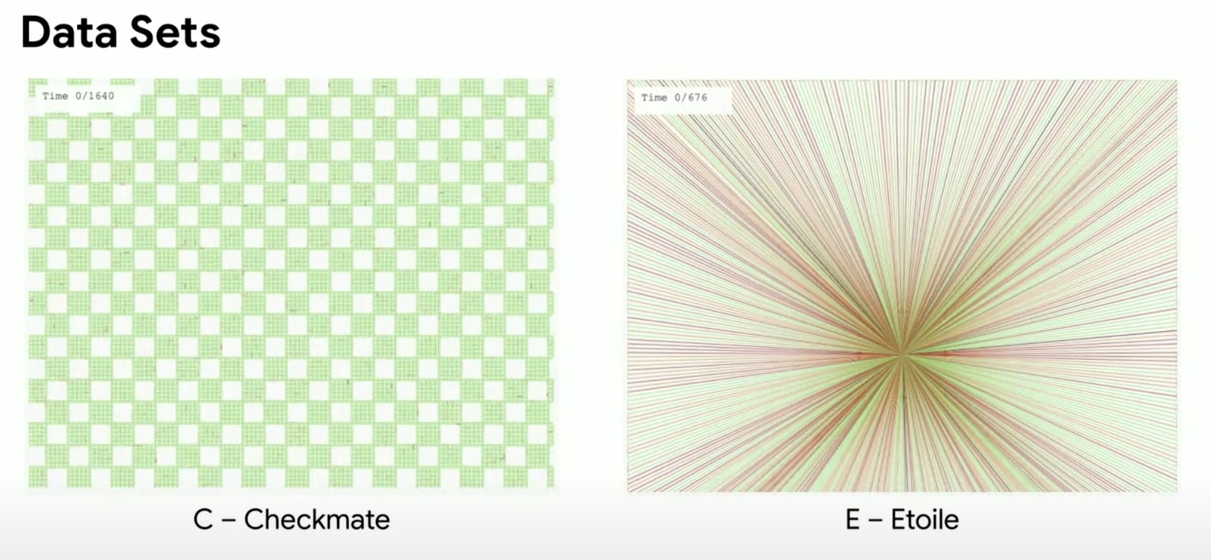
\includegraphics[width=\linewidth]{img/screenshots/hashcode_datasets_c_e.png}
    % 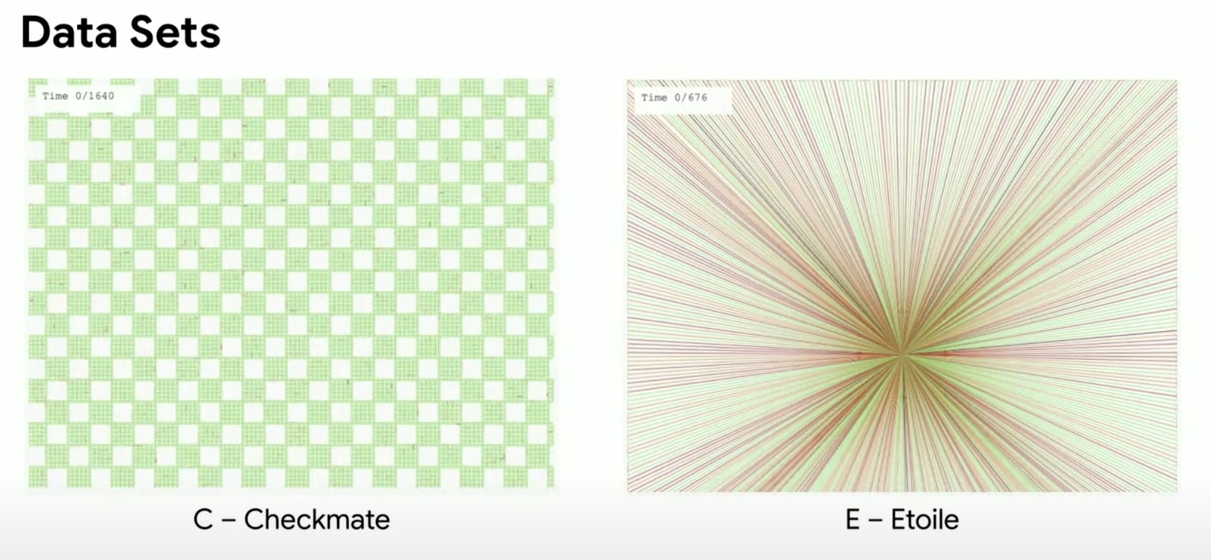
\includegraphics[width=.8\linewidth]{img/screenshots/hashcode_datasets_c_e.png}
    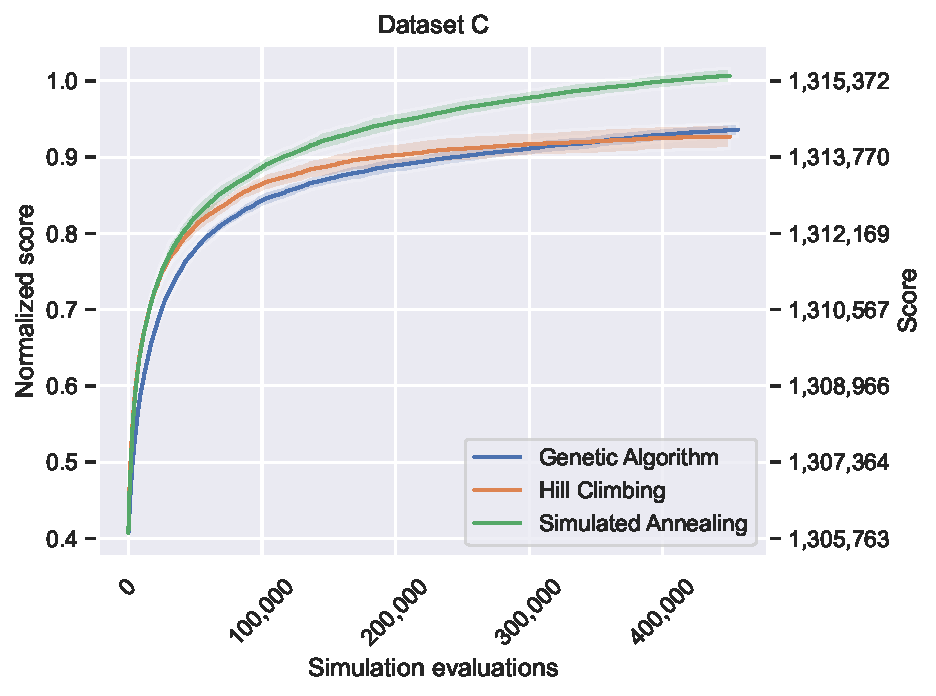
\includegraphics[width=\linewidth]{img/experiments/c_Genetic Algorithm_Hill Climbing_Simulated Annealing.pdf}
    \caption[Results for dataset C]{
        Results for dataset C.
    }
    \label{fig:dataset_c_experiment}
\end{figure}

\begin{figure}
    \centering
    % 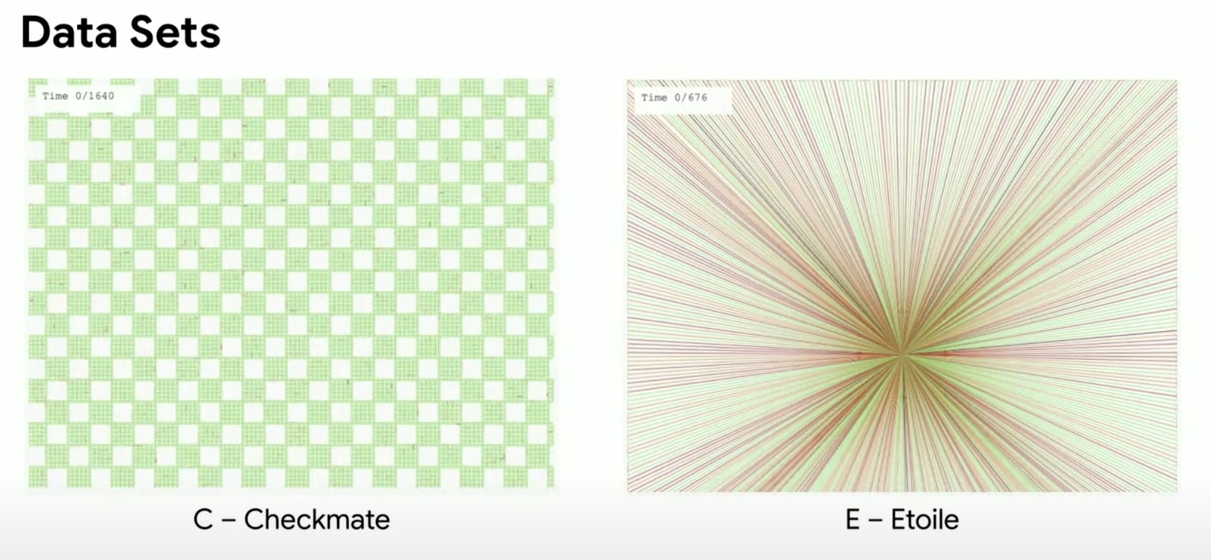
\includegraphics[width=\linewidth]{img/screenshots/hashcode_datasets_c_e.png}
    % 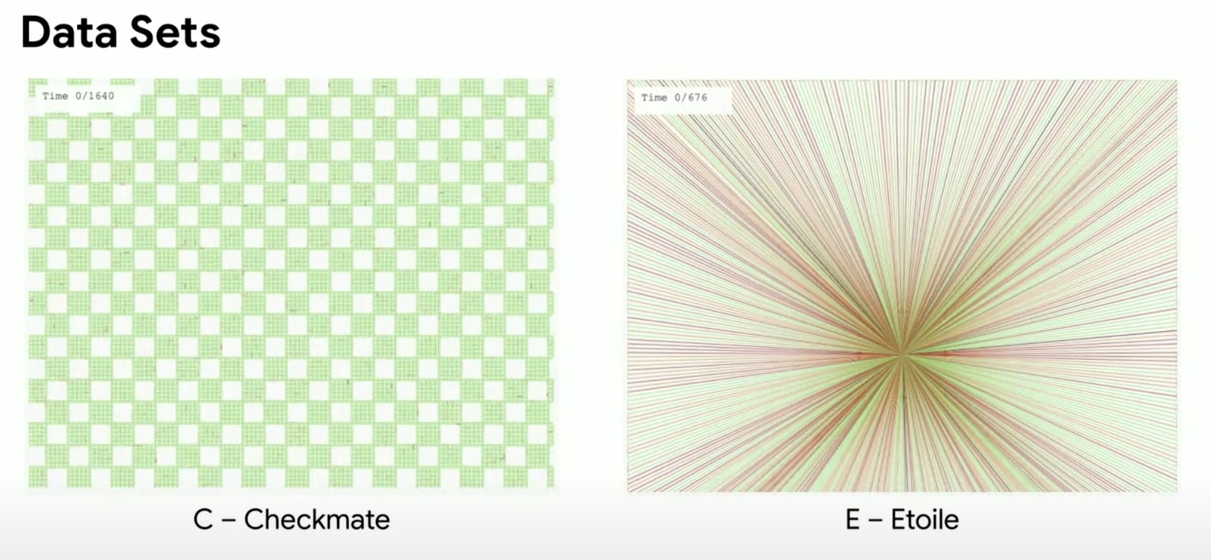
\includegraphics[width=.8\linewidth]{img/screenshots/hashcode_datasets_c_e.png}
    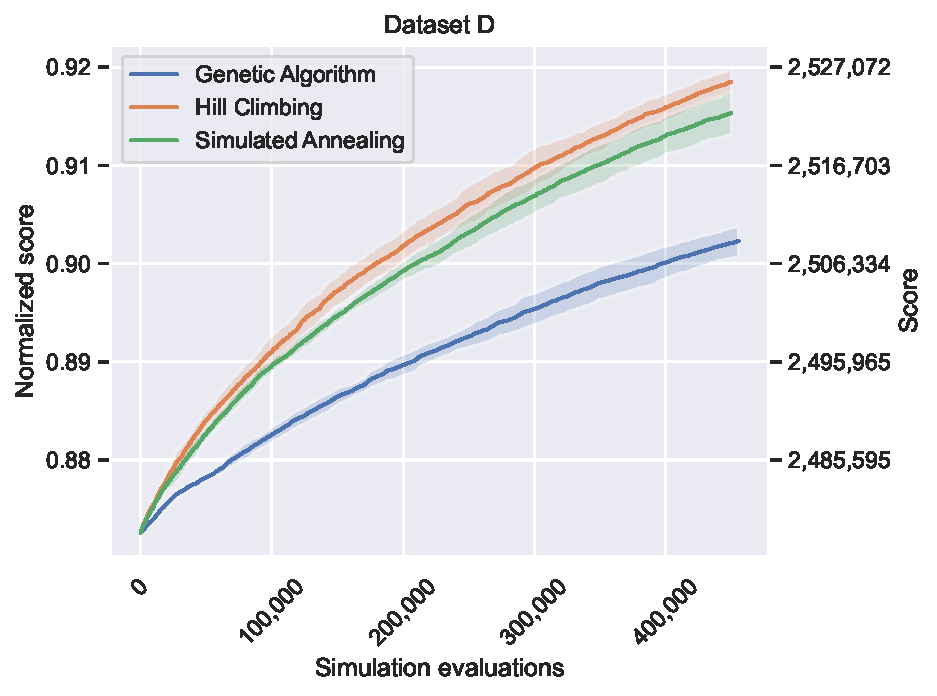
\includegraphics[width=\linewidth]{img/experiments/d_Genetic Algorithm_Hill Climbing_Simulated Annealing.pdf}
    \caption[Results for dataset D]{
        Results for dataset D.
    }
    \label{fig:dataset_d_experiment}
\end{figure}

\begin{figure}
    \centering
    % 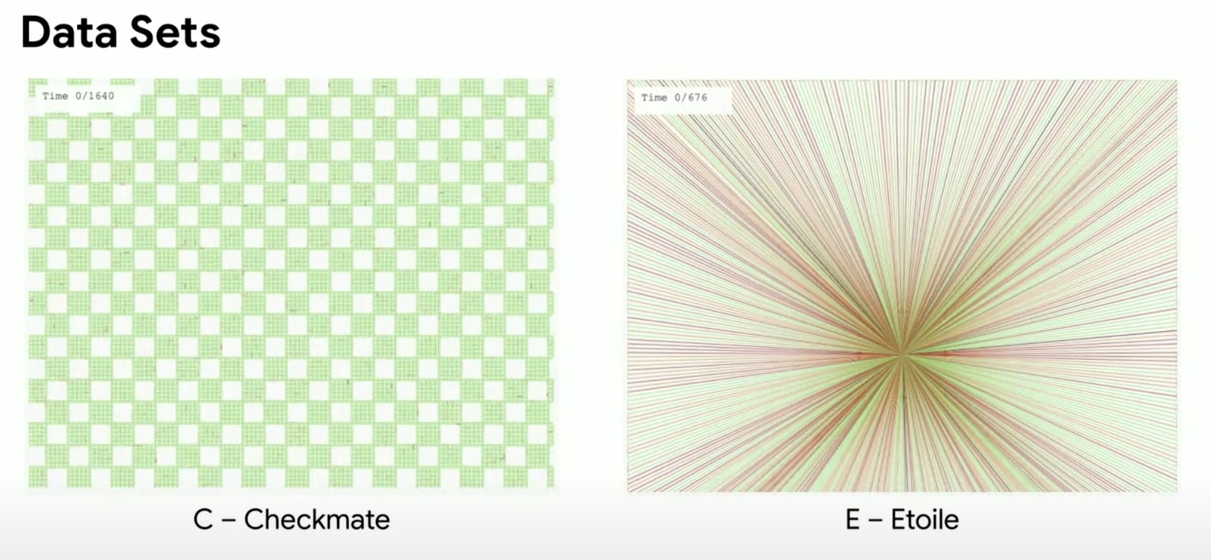
\includegraphics[width=\linewidth]{img/screenshots/hashcode_datasets_c_e.png}
    % 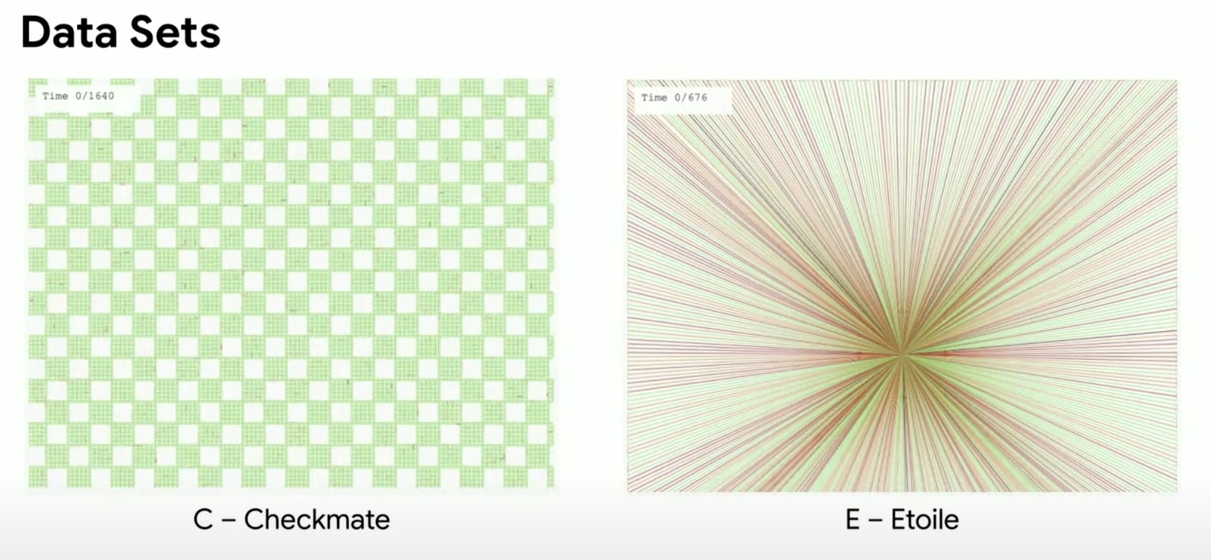
\includegraphics[width=.8\linewidth]{img/screenshots/hashcode_datasets_c_e.png}
    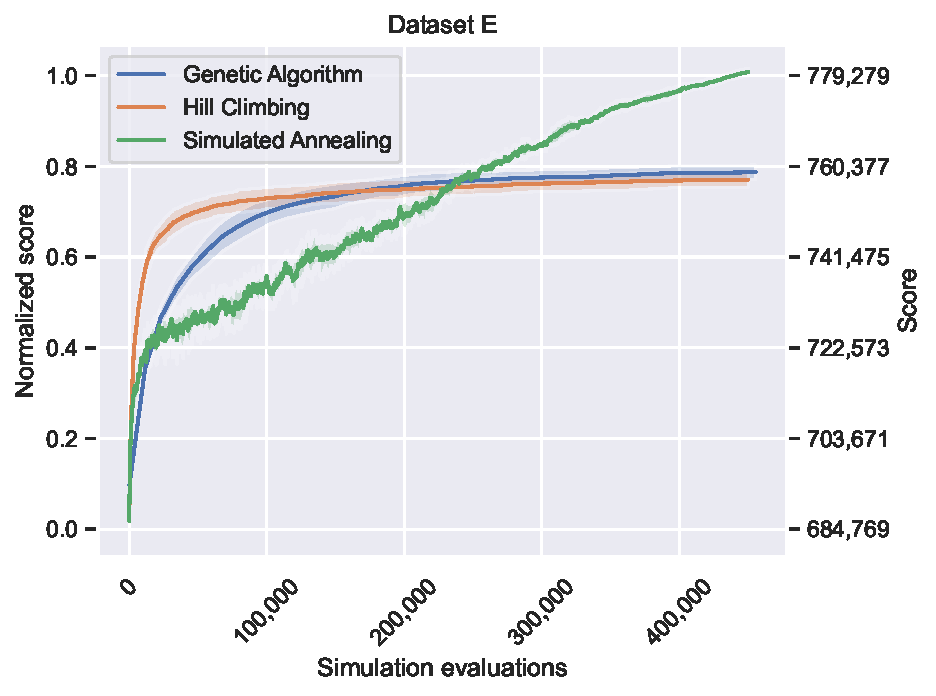
\includegraphics[width=\linewidth]{img/experiments/e_Genetic Algorithm_Hill Climbing_Simulated Annealing.pdf}
    \caption[Results for dataset E]{
        Results for dataset E.
    }
    \label{fig:dataset_e_experiment}
\end{figure}

\begin{figure}
    \centering
    % 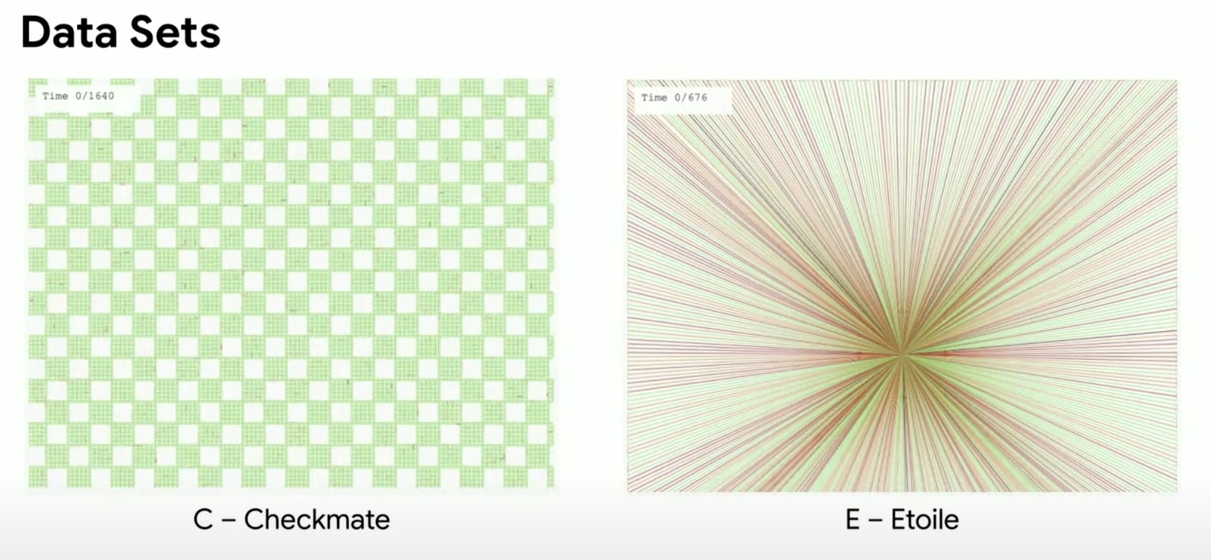
\includegraphics[width=\linewidth]{img/screenshots/hashcode_datasets_c_e.png}
    % 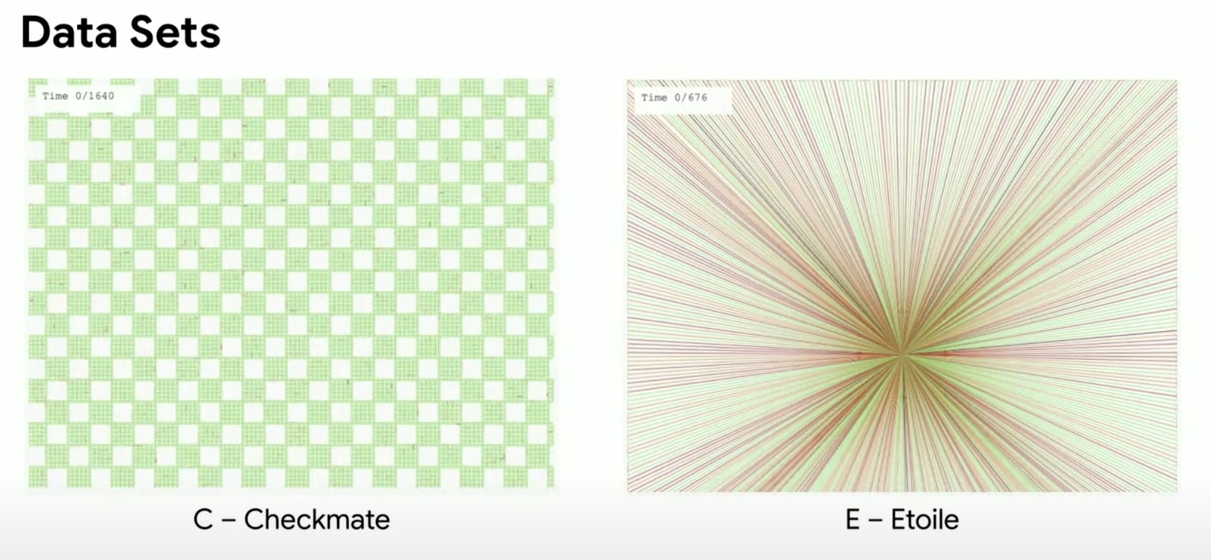
\includegraphics[width=.8\linewidth]{img/screenshots/hashcode_datasets_c_e.png}
    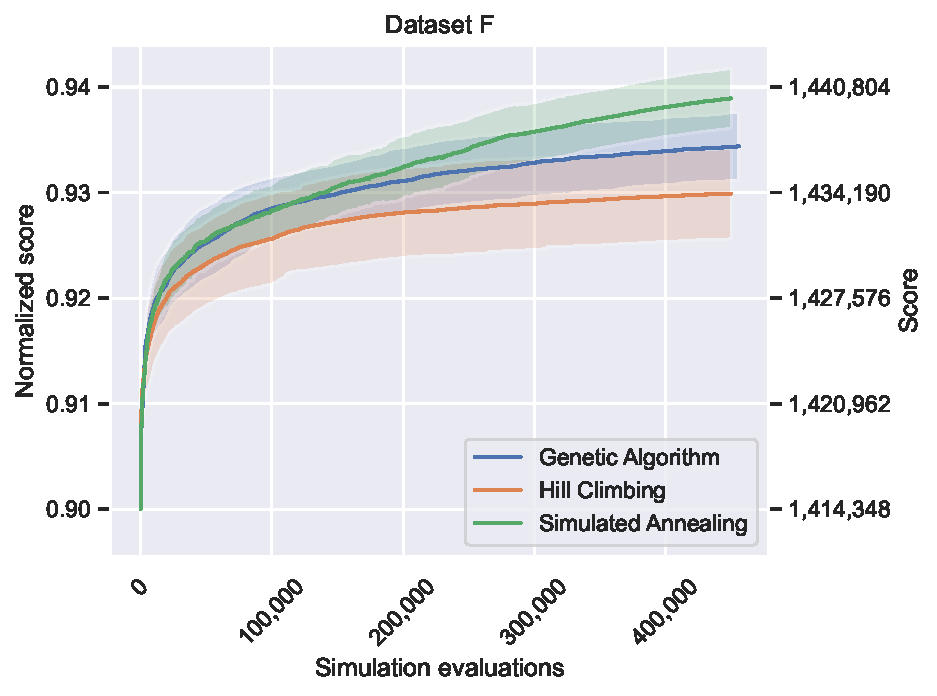
\includegraphics[width=\linewidth]{img/experiments/f_Genetic Algorithm_Hill Climbing_Simulated Annealing.pdf}
    \caption[Results for dataset F]{
        Results for dataset F.
    }
    \label{fig:dataset_f_experiment}
\end{figure}

% \begin{table}[b!]

% \centering
% %% Tabulka používá následující balíčky:
% %%   - booktabs (\toprule, \midrule, \bottomrule)
% %%   - dcolumn (typ sloupce D: vycentrovaná čísla zarovnaná na
% %%     desetinnou čárku
% %%     Všimněte si, že ve zdrojovém kódu jsou desetinné tečky, ale
% %%     tisknou se čárky.
% %% Dále používáme příkazy \pulrad a \mc definované v makra.tex

% \begin{tabular}{l@{\hspace{1.5cm}}D{.}{,}{3.2}D{.}{,}{1.2}D{.}{,}{2.3}}
% \toprule
%  & \mc{} & \mc{\textbf{Směrod.}} & \mc{} \\
% \pulrad{\textbf{Efekt}} & \mc{\pulrad{\textbf{Odhad}}} & \mc{\textbf{chyba}$^a$} &
% \mc{\pulrad{\textbf{P-hodnota}}} \\
% \midrule
% Abs. člen     & -10.01 & 1.01 & \mc{---} \\
% Pohlaví (muž) & 9.89   & 5.98 & 0.098 \\
% Výška (cm)    & 0.78   & 0.12 & <0.001 \\
% \bottomrule
% \multicolumn{4}{l}{\footnotesize \textit{Pozn:}
% $^a$ Směrodatná chyba odhadu metodou Monte Carlo.}
% \end{tabular}

% \caption{Maximálně věrohodné odhady v~modelu M.}\label{tab03:Nejaka}

% \end{table}

\begin{table}
% uncomment the following line if you use the fitted top captions for tables
% (see the \floatsetup[table] comments in `macros.tex`.
%\floatbox{table}[\FBwidth]{
\centering\footnotesize\sf
\begin{tabular}{llrl}
\toprule
Column A & Column 2 & Numbers & More \\
\midrule
Asd & QWERTY & 123123 & -- \\
Asd qsd 1sd & \textcolor{red}{BAD} & 234234234 & This line should be helpful. \\
Asd & \textcolor{blue}{INTERESTING} & 123123123 & -- \\
Asd qsd 1sd & \textcolor{violet!50}{PLAIN WEIRD} & 234234234 & -- \\
Asd & QWERTY & 123123 & -- \\
\addlinespace % a nice non-intrusive separator of data groups (or final table sums)
Asd qsd 1sd & \textcolor{green!80!black}{GOOD} & 234234299 & -- \\
Asd & NUMBER & \textbf{123123} & -- \\
Asd qsd 1sd & \textcolor{orange}{DANGEROUS} & 234234234 & (no data) \\
\bottomrule
\end{tabular}
%}{  % uncomment if you use the \floatbox (as above), erase otherwise
\caption{An example table.  Table caption should clearly explain how to interpret the data in the table. Use some visual guide, such as boldface or color coding, to highlight the most important results (e.g., comparison winners).}
%}  % uncomment if you use the \floatbox
\label{tab:z}
\end{table}

\begin{table}
% uncomment the following line if you use the fitted top captions for tables
% (see the \floatsetup[table] comments in `macros.tex`.
%\floatbox{table}[\FBwidth]{
\centering\footnotesize\sf
\begin{tabular}{llrl}
\toprule
Dataset & GA & HC & SA \\
\midrule
B & \textbf{0.95} & 0.90 & 0.85 \\
C & 0.90 & 0.88 & 0.87 \\
D & 0.98 & 0.96 & 0.95 \\
E & 0.92 & 0.91 & 0.89 \\
F & 0.93 & 0.90 & 0.88 \\
\bottomrule
% Asd & QWERTY & 123123 & -- \\
% Asd qsd 1sd & \textcolor{red}{BAD} & 234234234 & This line should be helpful. \\
% Asd & \textcolor{blue}{INTERESTING} & 123123123 & -- \\
% Asd qsd 1sd & \textcolor{violet!50}{PLAIN WEIRD} & 234234234 & -- \\
% Asd & QWERTY & 123123 & -- \\
% \addlinespace % a nice non-intrusive separator of data groups (or final table sums)
% Asd qsd 1sd & \textcolor{green!80!black}{GOOD} & 234234299 & -- \\
% Asd & NUMBER & \textbf{123123} & -- \\
% Asd qsd 1sd & \textcolor{orange}{DANGEROUS} & 234234234 & (no data) \\
% \bottomrule
\end{tabular}
%}{  % uncomment if you use the \floatbox (as above), erase otherwise
\caption{An example table.  Table caption should clearly explain how to interpret the data in the table. Use some visual guide, such as boldface or color coding, to highlight the most important results (e.g., comparison winners).}
%}  % uncomment if you use the \floatbox
\label{tab:results}
\end{table}

% TABLE WITH SHARED HYPERPARAMETERS
\begin{table}[h]
\centering\footnotesize\sf

\begin{tabular}{l@{}c}
% \toprule
\multicolumn{2}{l}{\textbf{Genetic Algorithm}} \\
Crossover probability & 0.6 \\
Mutation probability & 0.4 \\
Tournament size & 3 \\
Elitism & 0.05 \\
\midrule
\multicolumn{2}{l}{\textbf{Hill Climbing}} \\
Iterations & 450000 \\
\midrule
\multicolumn{2}{l}{\textbf{Simulated Annealing}} \\
Iterations & 450000 \\
% \bottomrule
\end{tabular}

\caption[Shared hyperparameters]{Shared hyperparameters across all datasets.}
\label{tab:hyperparams_shared}
\end{table}

% TABLE WITH DATASET-SPECIFIC HYPERPARAMETERS
\begin{table}[h]
\centering\footnotesize\sf

\begin{minipage}[t]{0.48\textwidth}
\centering
\begin{tabular}{l@{\hspace{0.5cm}}c}
% \toprule
\multicolumn{2}{c}{\textbf{Dataset E}} \\
\midrule
Order initialization & random \\
Times initialization & scaled \\
\midrule
\multicolumn{2}{l}{\textbf{Genetic Algorithm}} \\
Population size & 90 \\
Generations & 6667 \\
Mutation bit rate & 9 \\
\midrule
\multicolumn{2}{l}{\textbf{Hill Climbing}} \\
Mutation bit rate & 15 \\
\midrule
\multicolumn{2}{l}{\textbf{Simulated Annealing}} \\
Mutation bit rate & 5 \\
Initial temperature & 275 \\
% \bottomrule
\end{tabular}
\end{minipage}
\hfill
\begin{minipage}[t]{0.48\textwidth}
\centering
\begin{tabular}{l@{\hspace{0.5cm}}c}
% \toprule
\multicolumn{2}{c}{\textbf{Dataset B}} \\
\midrule
Order initialization & adaptive \\
Times initialization & default \\
\midrule
\multicolumn{2}{l}{\textbf{Genetic Algorithm}} \\
Population size & 10 \\
Generations & 60000 \\
Mutation bit rate & 2 \\
\midrule
\multicolumn{2}{l}{\textbf{Hill Climbing}} \\
Mutation bit rate & 4 \\
\midrule
\multicolumn{2}{l}{\textbf{Simulated Annealing}} \\
Mutation bit rate & 1 \\
Initial temperature & 0.25 \\
% \bottomrule
\end{tabular}
\end{minipage}
\newline
\newline
\newline
\begin{minipage}[t]{0.48\textwidth}
\centering
\begin{tabular}{l@{\hspace{0.5cm}}c}
% \toprule
\multicolumn{2}{c}{\textbf{Dataset F}} \\
\midrule
Order initialization & random \\
Times initialization & scaled \\
\midrule
\multicolumn{2}{l}{\textbf{Genetic Algorithm}} \\
Population size & 50 \\
Generations & 12000 \\
Mutation bit rate & 2 \\
\midrule
\multicolumn{2}{l}{\textbf{Hill Climbing}} \\
Mutation bit rate & 5 \\
\midrule
\multicolumn{2}{l}{\textbf{Simulated Annealing}} \\
Mutation bit rate & 3 \\
Initial temperature & 15 \\
% \bottomrule
\end{tabular}
\end{minipage}
\hfill
\begin{minipage}[t]{0.48\textwidth}
\centering
\begin{tabular}{l@{\hspace{0.5cm}}c}
% \toprule
\multicolumn{2}{c}{\textbf{Dataset C}} \\
\midrule
Order initialization & adaptive \\
Times initialization & default \\
\midrule
\multicolumn{2}{l}{\textbf{Genetic Algorithm}} \\
Population size & 20 \\
Generations & 30000 \\
Mutation bit rate & 2 \\
\midrule
\multicolumn{2}{l}{\textbf{Hill Climbing}} \\
Mutation bit rate & 4 \\
\midrule
\multicolumn{2}{l}{\textbf{Simulated Annealing}} \\
Mutation bit rate & 2 \\
Initial temperature & 0.1 \\
% \bottomrule
\end{tabular}
\end{minipage}
\newline
\newline
\newline
\begin{minipage}[t]{0.48\textwidth}
\centering
\begin{tabular}{l@{\hspace{0.5cm}}c}
% \toprule
\multicolumn{2}{c}{\textbf{Dataset D}} \\
\midrule
Order initialization & adaptive \\
Times initialization & default \\
\midrule
\multicolumn{2}{l}{\textbf{Genetic Algorithm}} \\
Population size & 40 \\
Generations & 15000 \\
Mutation bit rate & 2 \\
\midrule
\multicolumn{2}{l}{\textbf{Hill Climbing}} \\
Mutation bit rate & 2 \\
\midrule
\multicolumn{2}{l}{\textbf{Simulated Annealing}} \\
Mutation bit rate & 2 \\
Initial temperature & 0.1 \\
% \bottomrule
\end{tabular}
\end{minipage}

\caption[Dataset-specific hyperparameters]{
    Dataset-specific hyperparameters.
    The order and times initializations are the same for all three methods for each dataset.
}
\label{tab:hyperparams_datasets_specific}
\end{table}
